\chapter{Evaluation}\label{chapter:evaluation}

This chapter aims on presenting the concrete results that have been achieved using the respective approaches that were thoroughly explained in Chapter \ref{chapter:methodology} in order to provide an answer to the previously introduced research questions.

With regard to the visualization of the individual power measurements of the employed edge devices, the widgets of the constructed Grafana dashboard, which are illustrated by Figures \ref{fig:dashboard-total-power-consumption} - \ref{fig:dashboard-current}, provided an appropriate visualization of the data that was obtained using the employed PromQL queries that were introduced in the previous chapter. 

\begin{figure}[H]
    \centering
    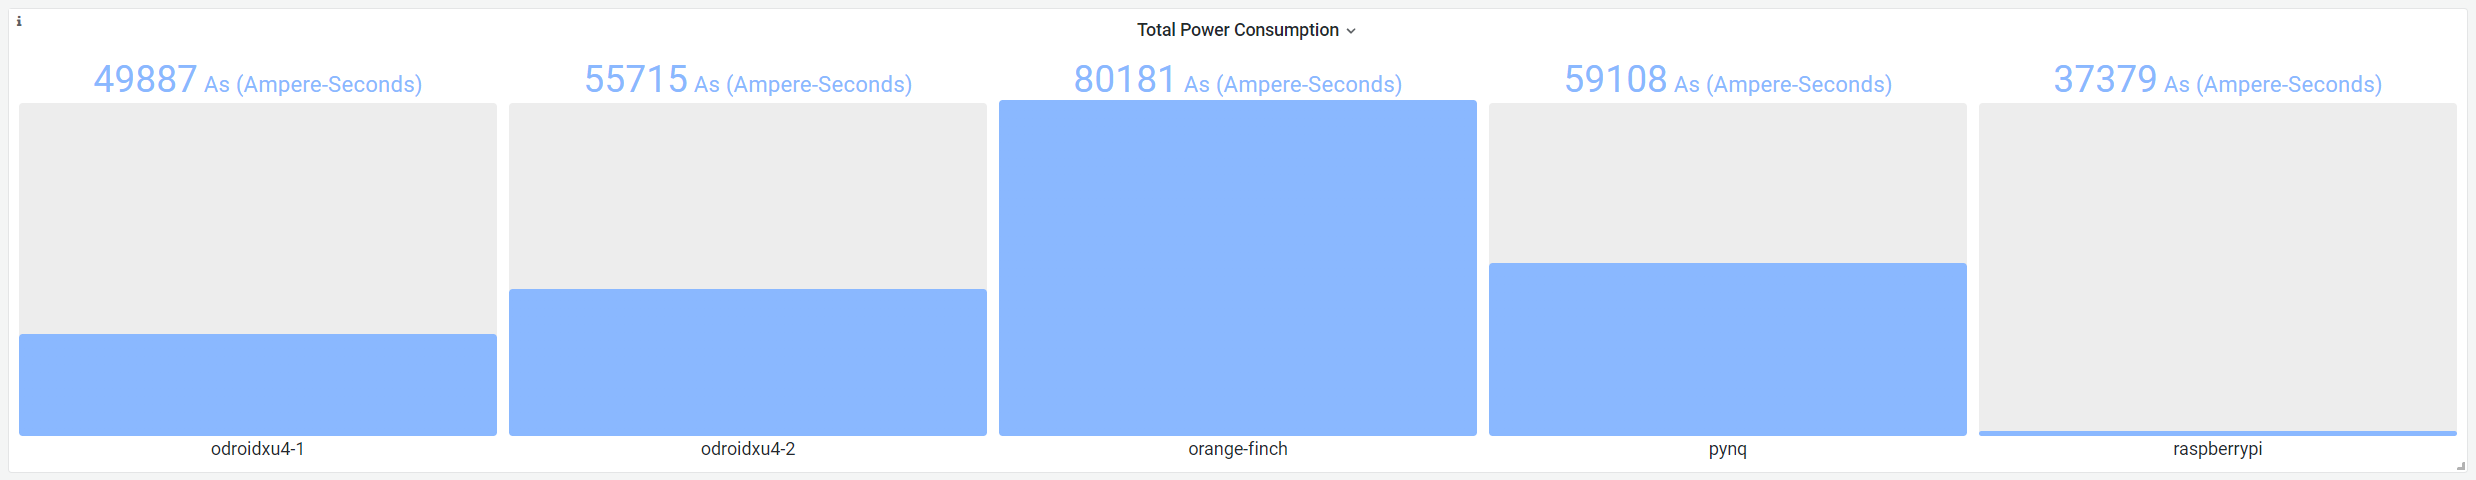
\includegraphics[width=\textwidth]{./figures/total_power_consumption}
    \caption{Visualization of the Total Energy Consumption per Edge-Device}
    \label{fig:dashboard-total-power-consumption}
\end{figure}

\begin{figure}[H]
    \centering
    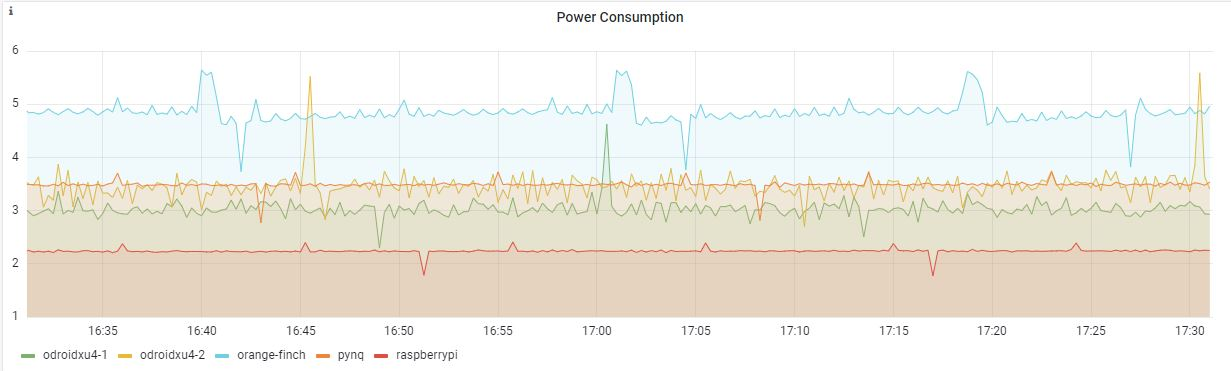
\includegraphics[width=\textwidth]{./figures/test}
    \caption{Visualization of the current Energy Consumption per Edge-Device}
    \label{fig:dashboard-power-consumption}
\end{figure}

\begin{figure}[H]
    \centering
    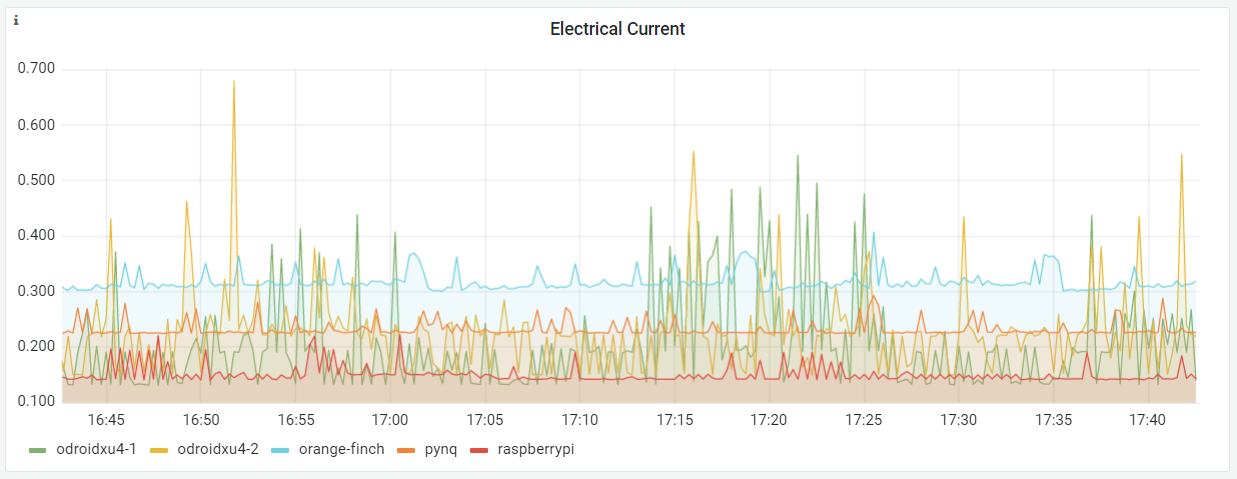
\includegraphics[width=\textwidth]{./figures/current}
    \caption{Visualization of the Electrical Current per Edge-Device}
    \label{fig:dashboard-current}
\end{figure}

